\section*{\Large{Введение}}
\addcontentsline{toc}{section}{\Large{Введение}}

% Основная мысль: вот пацаны смотрите какой генплан и он типа дофига сложный

Чтобы создать любой объект, необходимо сначала его представить.
Если объект достаточно простой, то весь процесс его создания может спокойно уместиться в голове человека.
Но по мере усложнения его устройства становится невозможно удержать весь контекст в голове,
процесс создания начинает требовать документации.
Когда объект становится совсем сложным, то его создание требует привлечения большого количества специалистов из разных
областей, знакомых с тонкостями той или иной сферы деятельности.

Описанное выше применимо и для сферы строительства.
Любому сложному строительству предшествует этап проектирования.
Результатом этого этапа является генеральный план площадного объекта (пример см. рис\ \ref{pic:introduction__site-plan}).
Именно на его основе проводится оценка, как капитальных, так и эксплуатационных затрат.
За проектирование крупных технологических объектов отвечают проектные институты,
а также инженеры-проектировщики, которые в них работают.

\begin{figure}[H]
	\vspace*{-0.4 cm}
	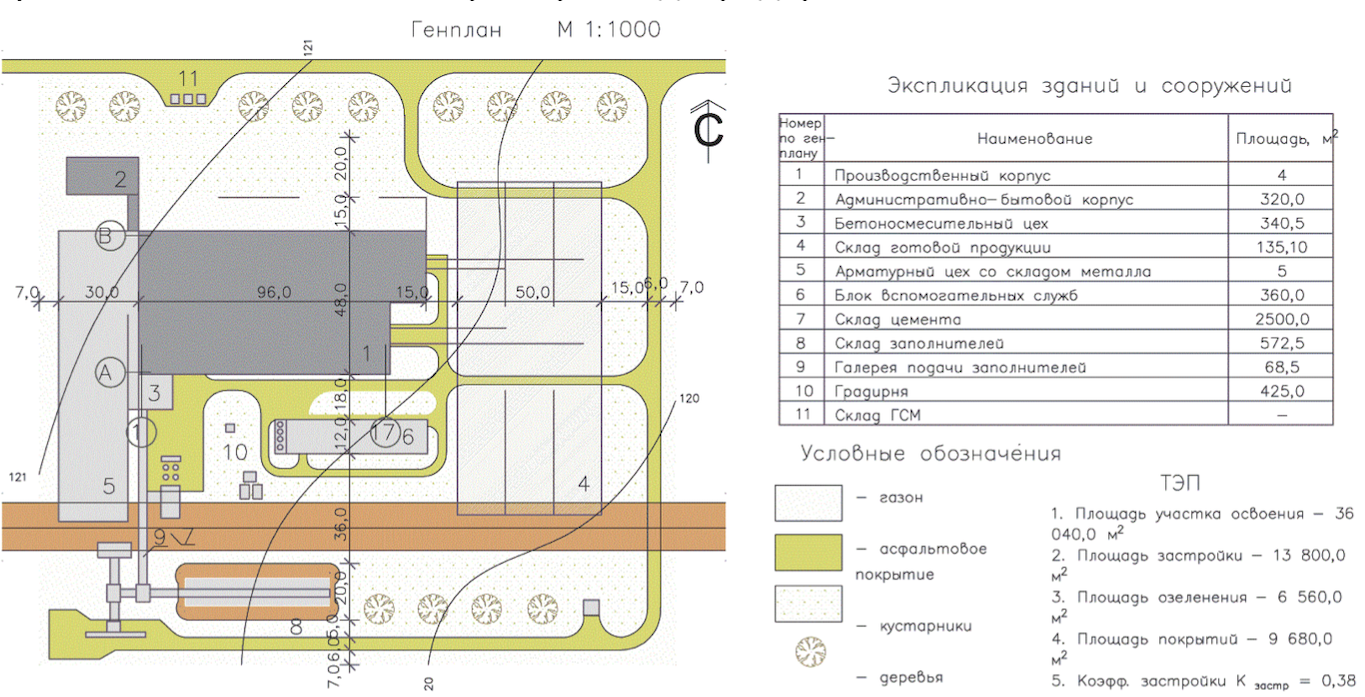
\includegraphics[width=0.8\textwidth]{introduction/pictures/site_plan}
	\caption{Пример генерального плана площадного объекта}
	\label{pic:introduction__site-plan}
\end{figure}
\vskip 5 mm

Основным рабочим инструментом для инженера-проектировщика являются системы автоматического проектирования.
В данных инструментах отсутствует возможность полностью автоматизировать процесс построения конструкции.
По сути, инженер строит решение вручную с нуля, базируясь на требованиях ГОСТ, СНиП, а также сводах правил
эксплуатации того или иного сооружения, что является сложным процессом, требующим высокой квалификации специалиста.
